%# -*- coding: utf-8-unix -*-
% !TEX program = xelatex
% !TEX root = ../thesis.tex
% !TEX encoding = UTF-8 Unicode
%%==================================================
%% chapter02.tex for SJTU Master Thesis
%% based on CASthesis
%% modified by wei.jianwen@gmail.com
%% Encoding: UTF-8
%%==================================================

\chapter{决策与规划}
\label{chap:chapter04}
运动规划(英语:Motion Planning)是一个过程,在考虑运动约束的同时寻找从起始状态到目标状态的移动步骤, 
其整体框架如图\ref{fig:motionplanning}所示 


\begin{figure}[!htp]
  \centering
  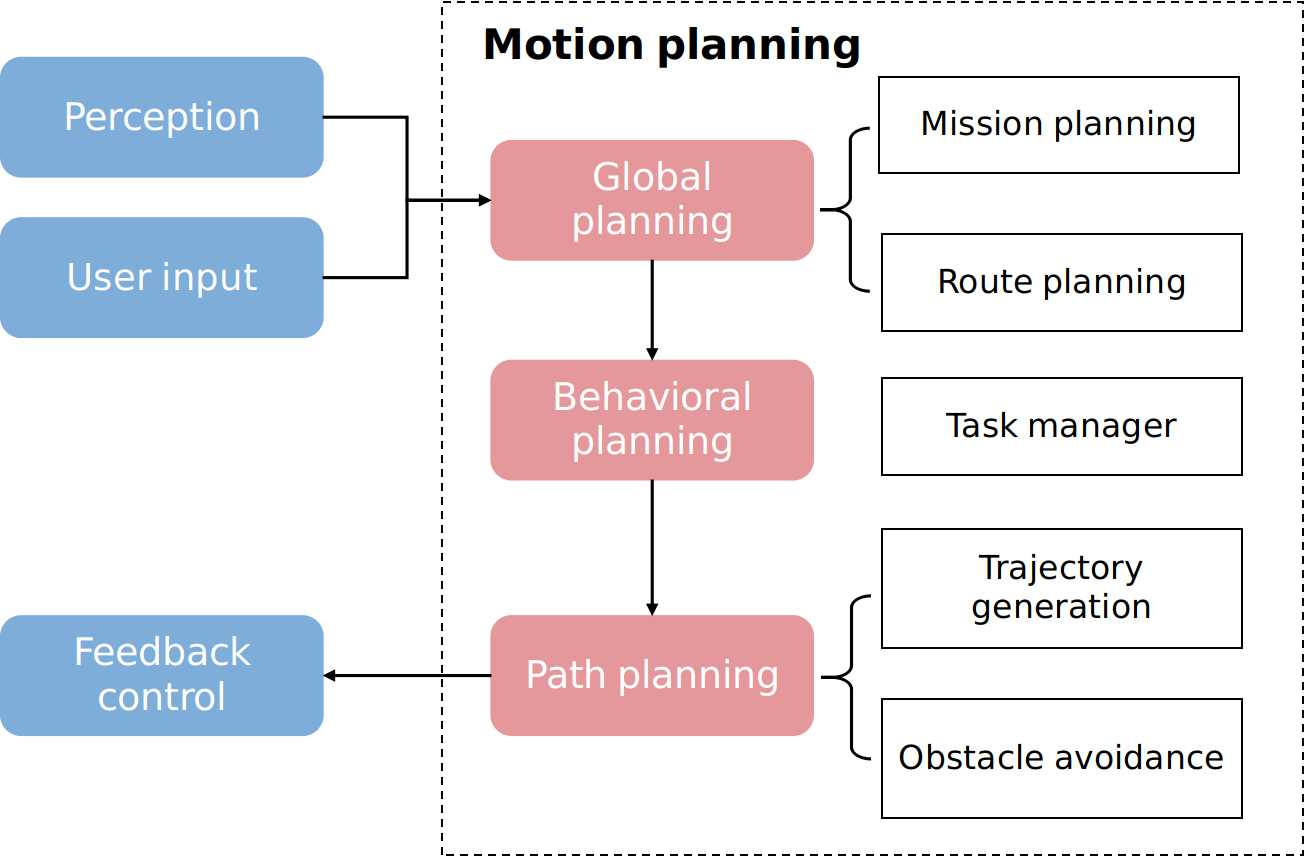
\includegraphics[width=13cm]{chapter04/motionplanning.jpg}
  \bicaption[运动规划的整体框架]
    {运动规划的整体框架}
    {Sketch of motion planning}
  \label{fig:motionplanning}
\end{figure}



\section{路径规划}
\label{sec:pathplanning}

\subsection{航道保持}
航道保持算法是无人船默认的局部路径规划算法, 其适用于中高速航行的船舶,同时可实现多种规划目标
(例如速度保持、超越、跟踪和停止等)。
\subsubsection{Jerk}
\begin{theorem}
\label{thm:jerktheorem}
给定初始时刻$t_0$的初始状态$P_0=[p_0, \dot{p}_0,\ddot{p}_0]$以及结束时刻$t_1= t_0+T$
的状态$P_1=[ \dot{p}_1,\ddot{p}_1]$, 五次多项式是下列惩罚函数的最优解,
\begin{equation}
  \begin{aligned}
    &C=k_j J_t + k_t g(T) + k_p h(p_1) \\
    &J_t(p(t)):=\int_{t_0}^{t_1} \dddot{p}^2(\tau) d \tau
  \end{aligned}
\end{equation}
其中,$g$和$h$是任意函数,$k_j, k_t, k_p>0$, $J_t$(Jerk)通常用于描述加加速度的积分,
其与交通工具的舒适程度有关。
\end{theorem}

\subsubsection{Frenet坐标系}
Frenet坐标系被广泛用于轨迹跟踪和轨迹生成算法中\cite{werling2010optimal}。
在Frenet坐标系中(见图\ref{fig:trajectoryfrenet}),我们以参考轨迹点为原点建立参考坐标系$(\bm{t}_r, \bm{n}_r)$,生成的轨迹点$\bm{x}(s(t),d(t))$可表示为
\begin{equation}
  \label{eq:frenetcoordinate}
  \bm{x}(s(t),d(t)) = \bm{r}(s(t)) + d(t) \cdot \bm{n_r}(s(t))
\end{equation}
表\ref{tab:frenetsymbol}列出了常用的符号,同时我们定义$\dot{(\cdot)}:=
\frac{\partial}{\partial t}(\cdot)$和$(\cdot)':=
\frac{\partial}{\partial s}(\cdot)$

\begin{table}[htbp]
  \centering
  \caption{符号解释}
    \begin{tabular}{ll}
    \toprule
    符号    & 物理含义 \\
    \midrule
    $t$          & 时间 \\
    $T$          & 时间间隔 \\
    $\bm{r}$     & 移动参考坐标系原点(即参考轨迹点)的笛卡尔坐标 \\
    $s$          & 参考轨迹点的弧坐标 \\
    $d$          & 生成轨迹点相对于参考轨迹点的横向偏移量 \\
    $\bm{t}_r$   & 移动参考坐标系的切向量 \\
    $\bm{n}_r$   & 移动参考坐标系的法向量 \\
    $\bm{t}_x$   & 生成轨迹点的切向量 \\
    $\bm{n}_x$   & 生成轨迹点的切向量 \\
    $\bm{x}$     & 生成轨迹的笛卡尔坐标 \\
    $\theta_r$   & 参考轨迹点的方向角 \\
    $\kappa_r$   & 参考轨迹点的曲率 \\
    $\theta_x$   & 生成轨迹点的方向角 \\
    $\kappa_x$   & 生成轨迹点的曲率 \\
    $v_x$  & 生成轨迹点的速度大小 \\
    $a_x$  & 生成轨迹点的加速度大小 \\
    \bottomrule
    \end{tabular}%
  \label{tab:frenetsymbol}%
\end{table}%

\begin{figure}[!htp]
  \centering
  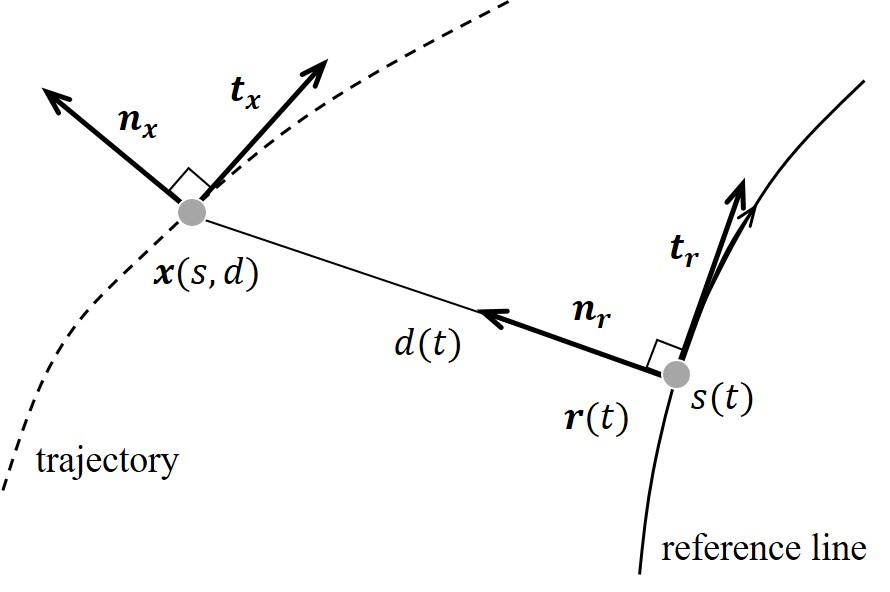
\includegraphics[width=10cm]{chapter04/trajectoryfrenet.jpg}
  \bicaption[Frenet坐标系下的轨迹生成]
    {Frenet坐标系下的轨迹生成}
    {Trajectory generation in a Frenet frame}
  \label{fig:trajectoryfrenet}
\end{figure}

\subsubsection{横向轨迹规划}
\begin{itemize}
  \item \textbf{中高速}

  给定横向的初始状态$D_0=[d_0, \dot{d}_0, \ddot{d}_0]$, 我们假设$\dot{d}_1=\ddot{d}_1=0$
  (这也是我们期望的最终状态),并假设$g(T)=T, \quad h(d_1)=d_1^2$, 由此可得
  \begin{equation}
    C_d = k_j J_t(d(t))+k_t T + k_d d_1^2
  \end{equation}
  $C_d$中最后一项用于惩罚最终状态$d \neq 0$的情况。由定理\ref{thm:jerktheorem}可得,
  $d(t)$是关于$t$的五次多项式(quintic polynomials)。通过调整最终状态的$d_i$和$T_j$
  \begin{equation}
    [d_1,\dot{d}_1,\ddot{d}_1,T]_{ij}=[d_i,0,0,T_j]
  \end{equation}
  注意,船体的状态是实时变化的,因此$D_0$始终表示船体当前时刻的状态,相应的$D_1$表示规划的
  最终状态,也是实时变化的。

  \item \textbf{低速}

  对于中高速的情况下,$s(t)$和$d(t)$可以被分开计算;但对于低速的情况,对$s(t)$和$d(t)$
  独立处理的方法违背了刚体运动的non-holonomic的性质,因此横向轨迹的计算需要考虑纵向轨迹
  \begin{equation}
    \bm{x}(s(t),d(t)) = \bm{r}(s(t)) + d(s(t)) \cdot \bm{n}_r(s(t))
  \end{equation}
  考虑低速的情形,我们修改了惩罚函数
  \begin{equation}
    \begin{aligned}
      &C_d = k_j J_s(d(s)) + k_t S + k_d d_1^2 \\
      &J_s(d(s)):= \int_{s_0}^{s_1} d'''^2(\sigma) d \sigma
    \end{aligned}
  \end{equation}
  该惩罚函数的最优值是$d(s)$关于$s$的五次多项式,且该多项式的初始点$D_0=[d_0, d'_0, d''_0]$
  和终止点为
  \begin{equation}
    [d_1, d'_1,d''_1, T]_{ij}=[d_i, 0, 0, T_j]
  \end{equation}
\end{itemize}

\subsubsection{纵向轨迹规划}
对于纵向的轨迹规划,主要分为跟踪、超越、速度保持和停止。
\begin{itemize}
  \item \textbf{速度保持}

  未感知到障碍物的时候,我们希望船舶匀速航行。结合$s_1$的Transversality condition
  \cite{IROS637936}和定理\ref{thm:jerktheorem},可知四次多项式(quartic polynomials)能够
  使得以下惩罚函数最小,
  \begin{equation}
    C_v = k_j J_t(s(t)) + k_t T + k_{\dot{s}}[\dot{s}_1-\dot{s}_d]^2
  \end{equation}
  其中,我们给定$t_0$时刻$S_0=[s_0, \dot{s}_0, \ddot{s}_0]$,$t_1=t_0+T$时刻的状态
  $S_1=[\dot{s}_1,\ddot{s}_1]$。这就意味着,$s$可以用$t$的四次多项式表示,而多项式的
  初始条件分别为$S_0=[s_0, \dot{s}_0, \ddot{s}_0]$和以下终止条件
  \begin{equation}
    [\dot{s}_1, \ddot{s}_1, T]_{ij}= [\dot{s}_d+\Delta \dot{s}_i, 0, T_j]
  \end{equation}
  当我们调整$\Delta \dot{s}_i$和$T_j$时,可得不同终止条件下的轨迹。
  \item \textbf{跟踪}

  对于跟踪、超越和停止的情况,都存在目标的位置$s_{target}(t)$,给定了$S_0 = [s_0,
  \dot{s}_0, \ddot{s}_0]$和以下的终止条件
  \begin{equation}
    [s_1, \dot{s}_1,\ddot{s}_1, T]_{ij}=[s_{target}(T_j)+\Delta s_i \: ,
    \dot{s}_{target}(T_j) \: , \ddot{s}_{target}(T_j) \: , T_j]
  \end{equation}
  可得$s(t)$关于$t$的五次多项式是以下惩罚函数(cost function)的最优解,
  \begin{equation}
    C_t = k_j J_t + k_t T + k_s(s_1-s_d)^2
  \end{equation}
  当我们调整终止条件中的$\Delta s_i$和$T_j$,可得多条纵向轨迹。

  对于跟踪,也就是与前方的船舶保持一定的距离,这个距离也需要满足海事规范,
  \begin{equation}
    s_{target}(t):=s_{lv}(t)-(D_0+\tau \dot{s}_{lv}(t))
  \end{equation}
  其中,$D_0$和$\tau$是常数,$s_{lv}$和$\dot{s}_{lv}$分别是领导船只沿轨迹线的位置和速度。
  \item \textbf{超越和停止}

  \begin{equation}
    s_{target}(t)=\frac{1}{2}[s_a(t)+s_b(t)]
  \end{equation}
  其中$s_a(t)$和$s_b(t)$分别是周围两条船的位置。对于停止的情况,
  $s_{target}=s_{stop} \, , \, \dot{s}_{target}=0 \, , \, \ddot{s}_{target}=0$
\end{itemize}

\subsubsection{轨迹结合}
通过调整终止条件,我们可得横向和纵向的多项式线束(Lattice),$\Pi_{lat}$和$\Pi_{lon}$,
从而生成轨迹线束$\Pi_{lat} \times \Pi_{lon}$,如图\ref{fig:frenetlattice}所示。在选取
最优轨迹的过程中,我们考虑联合惩罚函数$C_{tot}=k_{lat}C_{lat}+k_{lon}C_{lon}$, 同时保证
生成轨迹与障碍物有一定的安全距离。最终保证避障的条件下,选取最优轨迹。

\begin{figure}[!htp]
  \centering
  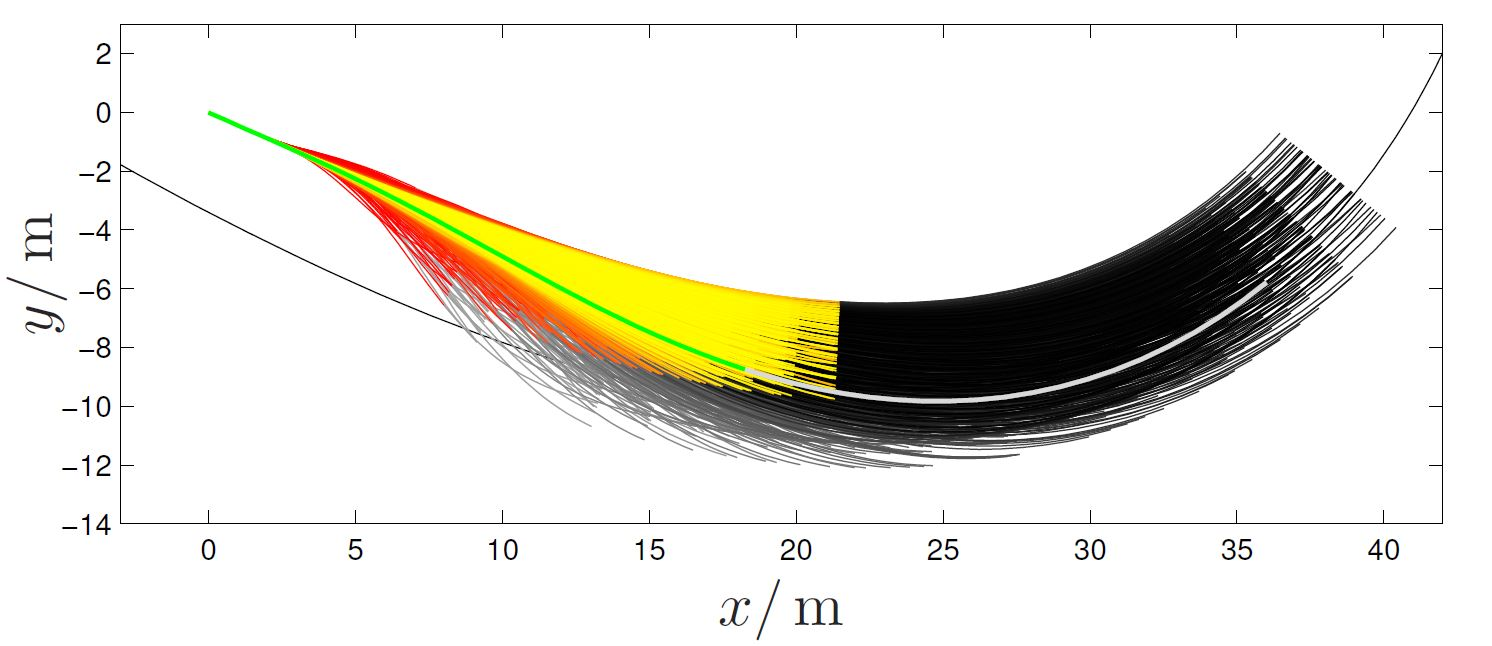
\includegraphics[width=12cm]{chapter04/frenetlattice.jpg}
  \bicaption[Frenet坐标系下的最优轨迹线束]
    {Frenet坐标系下的最优轨迹线束, 其预测时间为3秒,红色到黄色代表递增的惩罚值(cost),
    当障碍物不存在时,“绿-灰”的轨迹即为最优轨迹,使得船体回归参考轨迹。}
    {Resulting trajectory set in global coordinates for velocity keeping: The color map visualizes the increasing costs of both the reactive layer with 3.0 s lookahead from red to yellow and the alternatives for the long-term objectives form gray to black. As there are no obstacles within the 3.0 s horizon, the optimal trajectory of the free problem is chosen (green, light gray), which leads the vehicle back to the center line and to the desired speed.
    }
  \label{fig:frenetlattice}
\end{figure}


\subsubsection{坐标转换}
计算轨迹线束时,需要Frenet坐标系和Cartesian坐标系的相互转换。Frenet坐标系下的船体状态为
$ [s, \dot{s}, \ddot{s} \,; d, \dot{d},\ddot{d}/d, d', d'']$和$[\bm{x}, \theta_x, \kappa_x, v_x, a_x]$,首先我们推导一些通用的公式。

我们定义$\bm{t}_r(s):=[\cos(\theta_r(s)) \: \sin(\theta_r(s))]^T$,
$\bm{n}_r(s):=[ -\sin(\theta_r(s)) \: \cos(\theta_r(s))]^T$和
$\Delta \theta:=\theta_x - \theta_r$,且确保$|\Delta \theta| < \frac{\pi}{2}$和
$1-\kappa_r d >0$。
由Frenet-Serret公式可得
\begin{equation}
  \begin{aligned}
    &\frac{\mathrm{d} \bm{n}_r}{\mathrm{d} s} = -{\kappa}_r \bm{t}_r, \quad
    \frac{\mathrm{d} \bm{n}_r}{\mathrm{d} t} = -\dot{s}{\kappa}_r \bm{t}_r \\
    &\frac{\mathrm{d} \bm{t}_r}{\mathrm{d} s} = {\kappa}_r \bm{n}_r, \quad
    \frac{\mathrm{d} \bm{t}_r}{\mathrm{d} t} = \dot{s} {\kappa}_r \bm{n}_r
  \end{aligned}
\end{equation}
结合Frenet-Serret公式,由方程\ref{eq:frenetcoordinate}可得
\begin{equation}
  d=[\bm{x}-\bm{r}(s)]^T \cdot \bm{n}_r
\end{equation}
对上式作时间的导数,可得
\begin{equation}
  \begin{aligned}
    \dot{d}
    &=[\dot{\bm{x}}-\dot{\bm{r}}(s)]^T \bm{n}_r +
            [\bm{x}-\bm{r}(s)]^T \dot{\bm{n}}_r \\
    &=v_x \bm{t}_x^T \bm{n}_r - \dot{s} \bm{t}_r^T \bm{n}_r - \dot{s} {\kappa}_r
    [\bm{x}-\bm{r}(s)]^T \bm{t}_r \\
    &= v_x \sin(\Delta \theta)
  \end{aligned}
\end{equation}
同时,我们得到
\begin{equation}
  \begin{aligned}
    v_x
    &= || \dot{\bm{x}} ||_2 \\
    &= || \dot{\bm{r}}(s) + \dot{d} \bm{n}_r +d \dot{\bm{n}}_r ||_2 \\
    &= || \dot{s}\bm{t}_r + \dot{d} \bm{n}_r - \dot{s} {\kappa}_r d \bm{t}_r ||_2 \\
    &= \left\|
        \left[
          \begin{array}{cc}
            {\bm{t}_{r}} & {\bm{n}_{r}}
          \end{array}
        \right]
        \left[
          \begin{array}{cc}
            {1-\kappa_{r} d} & {0} \\ {0} & {1}
          \end{array}
        \right]
        \left[
          \begin{array}{c}
            {\dot{s}} \\ {\dot{d}}
          \end{array}
        \right]
      \right\|_2 \\
    &= \sqrt{(1-{\kappa}_r d)^2 \dot{s}^2 +\dot{d}^2}
  \end{aligned}
\end{equation}
且
\begin{equation}
  \label{eq:ddds}
  \begin{aligned}
    d'
    &=\frac{\mathrm{d} t}{\mathrm{d} s} \frac{\mathrm{d} }{\mathrm{d} t} d
    =\frac{\dot{d}}{\dot{s}} = \frac{1}{\dot{s}} v_x \sin(\Delta \theta) \\
    &=\sqrt{(1-{\kappa}_r d)^2 +d'^2}  \sin(\Delta \theta) \\
    & \Rightarrow \\
    d'
    &=(1-{\kappa}_rd) \tan(\Delta \theta)
  \end{aligned}
\end{equation}
已知$(\bm{x}-\bm{r}(s))^T \bm{t}_r = 0$,对其作时间导数可得 $  \frac{v_x}{\dot{s}} \cos(\Delta \theta) -1 + {\kappa}_r d = 0$, 变化得到船体的速度大小
\begin{equation}
  v_x = \dot{s} \frac{1-{\kappa}_r d}{\cos(\Delta \theta)}
\end{equation}
我们用$s_x$表示轨迹$\bm{x}$上的弧长,根据曲率的定义${\kappa_x}=\frac{\mathrm{d} \theta_x}{\mathrm{d}s_x}$和${\kappa_r}=\frac{\mathrm{d} \theta_r}{\mathrm{d}s}$,
可得
\begin{equation}
  \frac{\mathrm{d}}{\mathrm{d}s} =\frac{\mathrm{d} s_x}{\mathrm{d}t}
  \frac{\mathrm{d} t}{\mathrm{d} s} \frac{\mathrm{d}}{\mathrm{d}s_x}
  = \frac{v_x}{\dot{s}} \frac{\mathrm{d}}{\mathrm{d}s_x}
  =\frac{1-{\kappa}_r d}{\cos(\Delta \theta)} \frac{\mathrm{d}}{\mathrm{d}s_x}
\end{equation}
\begin{equation}
  \begin{aligned}
    \Delta \theta ' = \frac{\mathrm{d}( {\theta}_x - {\theta}_r)}{\mathrm{d}s}
    &= \frac{\mathrm{d}}{\mathrm{d} s} {\theta}_x - {\kappa}_r \\
    &= \frac{1-{\kappa}_r d}{\cos(\Delta \theta)} {\kappa}_x - {\kappa}_r  \\
  \end{aligned}
\end{equation}
由公式\ref{eq:ddds},我们可得$d$对$s$的二阶导数
\begin{equation}
  d''=-({\kappa}_r  d)' \tan(\Delta \theta) + \frac{1-{\kappa}_r d}
  {\cos^2(\Delta \theta)}    \Delta \theta '
\end{equation}
将速度$v_x$对时间求导可得
\begin{equation}
  a_x := \dot{v}_x = \ddot{s}\frac{1-{\kappa}_r d}{\cos(\Delta \theta)}  +
  \frac{\dot{s}^2}{\cos(\Delta \theta)}[d' \Delta \theta' - ({\kappa}_r d)']
\end{equation}
同时, $s$对时间$t$的二阶导数
\begin{equation}
  \ddot{s}=\frac{a_x \cos(\Delta \theta)- \dot{s}^2
  [d' \Delta \theta' - ({\kappa}_r d)']}{1-{\kappa}_r d}
\end{equation}
在中高速的情况下($d$与$s$无关),
\begin{equation}
  \begin{aligned}
    &\dot{d}=\frac{\mathrm{d}}{\mathrm{d} t}d=\frac{\mathrm{d}s}{\mathrm{d} t}
    \frac{\mathrm{d}}{\mathrm{d} s}d= \dot{s}d' \\
    &\ddot{d}=d'' \dot{s}^2 + d' \ddot{s}
  \end{aligned}
\end{equation}


坐标系之间的转换将会用于Frenet Lattice的实时计算中(如图\ref{fig:frenetalgorithm}),
下面我们分别讨论两个坐标系之间的转换过程
\begin{itemize}
  \item \textbf{从Cartesian到Frenet}

  给定船体当前时刻的状态为$[\bm{x},\theta_x, \kappa_x, v_x, a_x](t_0)$, 我们希望得到
  在Frenet坐标系下,当前时刻的状态$[s_0, \dot{s}_0, \ddot{s}_0, d_0, \dot{d}_0,
  \ddot{d}_0]$或者$[s_0, \dot{s}_0, \ddot{s}_0, d_0, d'_0, d''_0]$。
  \begin{equation}
    [\bm{x}, \theta_x, \kappa_x, v_x, a_x]  \rightarrow
    [s, \dot{s}, \ddot{s}; d, \dot{d},\ddot{d}/d, d', d'']
  \end{equation}
  首先,采用一些高效的数值方法得到船体在参考轨迹上的投影点$s$
  \begin{equation}
    s= arg\,min_{\sigma} || \bm{x}-\bm{r}(\sigma)||
  \end{equation}
  得到$s$之后,根据参考轨迹的多项式公式,可得${\kappa}_r, {\kappa}'_r$和${\theta}_r$,
  从而计算$\Delta \theta = {\theta}_x-{\theta}_r $, 剩下的变量也可以根据以上公式推导
  得到。

  \item \textbf{从Frenet到Cartesian}

  当我们得到生成轨迹$[s, \dot{s}, \ddot{s}; d, \dot{d},\ddot{d}/d, d', d'']$的时候,
  需要得出Cartesian坐标系中,生成轨迹的状态
  \begin{equation}
    [s, \dot{s}, \ddot{s}; d, \dot{d},\ddot{d}/d, d', d''] \rightarrow
    [\bm{x}, \theta_x, \kappa_x, v_x, a_x]
  \end{equation}

\end{itemize}

\begin{figure}[!htp]
  \centering
  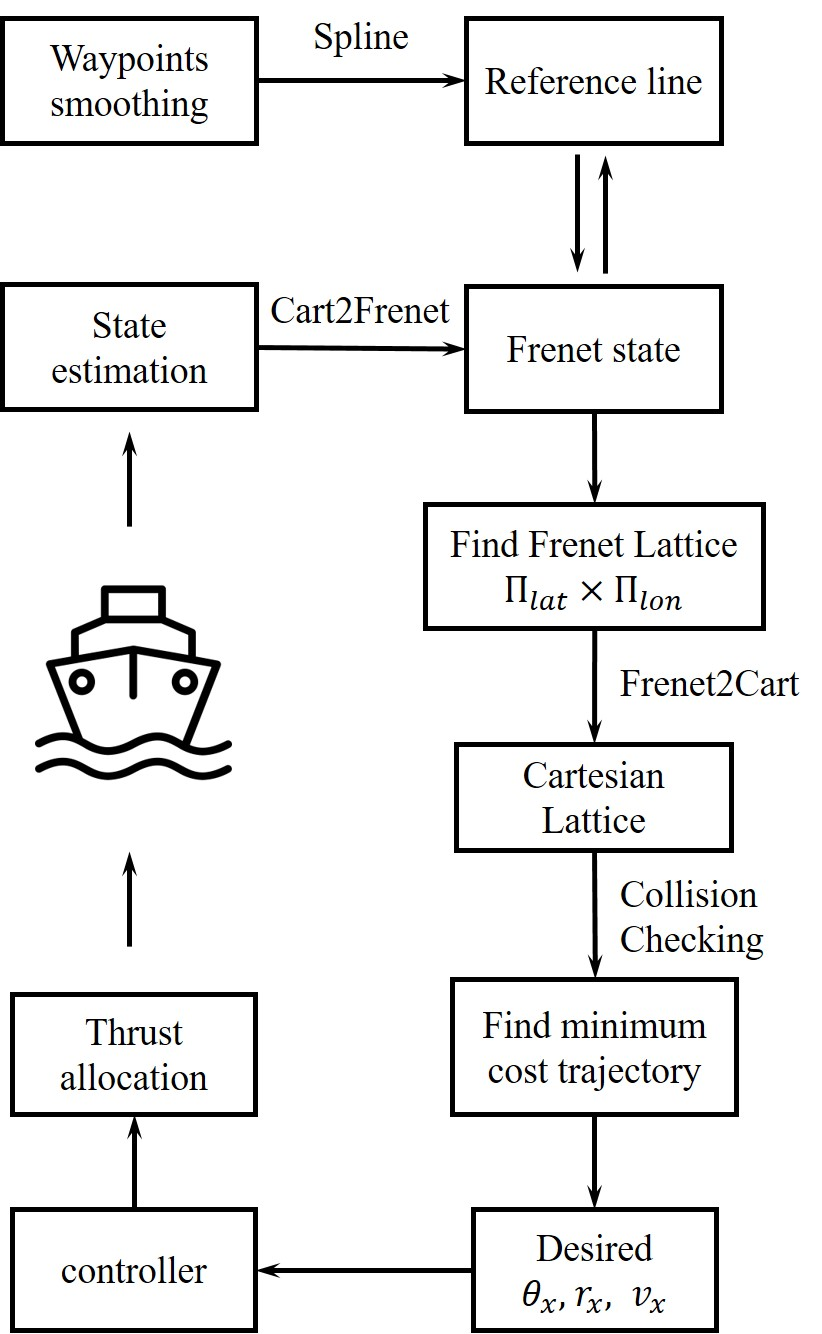
\includegraphics[width=15cm]{chapter04/Algorithm.jpg}
  \bicaption[Frenet坐标系下的最优轨迹生成算法逻辑图]
    {Frenet坐标系下的最优轨迹生成算法逻辑图}
    {Flowchart for trajectory generator in the Frenet frame}
  \label{fig:frenetalgorithm}
\end{figure}


\subsection{低速泊船}
自动停车是一种自动驾驶汽车的系统,它将车辆从行车道移入停车位,以执行平行,垂直或角度停车。适用于低速。

\subsubsection{Reeds-Shepp曲线}
对于欠驱动的机器人(nonholonomic system),其运动模型为

\begin{equation}
  \begin{aligned}
    & x(t)=x(0)+\int_0^t \varepsilon( \tau ) \cos \phi (\tau) \mathrm{d} \tau   \\
    & y(t)=y(0)+\int_0^t \varepsilon( \tau ) \sin \phi (\tau) \mathrm{d} \tau   \\
    & \phi (t)= \phi (0) + \int_0^t \eta (\tau) \mathrm{d} \tau
  \end{aligned}
\end{equation}

其中,$\gamma(t)=[x(t), y(t), \phi(t)]$为机器人的可行轨迹。

如何找到一条最短的路径把船从一个地方开到另外一个地方。答案就是图\ref{fig:rscurve}所示的
Reeds-Shepp曲线\cite{reeds1990} 。
假设车辆能以固定的半径转向,且车辆能够前进和后退,
那么Reeds-Shepp曲线就是车辆在上述条件下从起点到终点的最短路径。
该曲线不仅能保证车辆能够到达终点,而且能保证车辆的角度能在终点到达预期角度。


\begin{figure}[!htp]
  \centering
  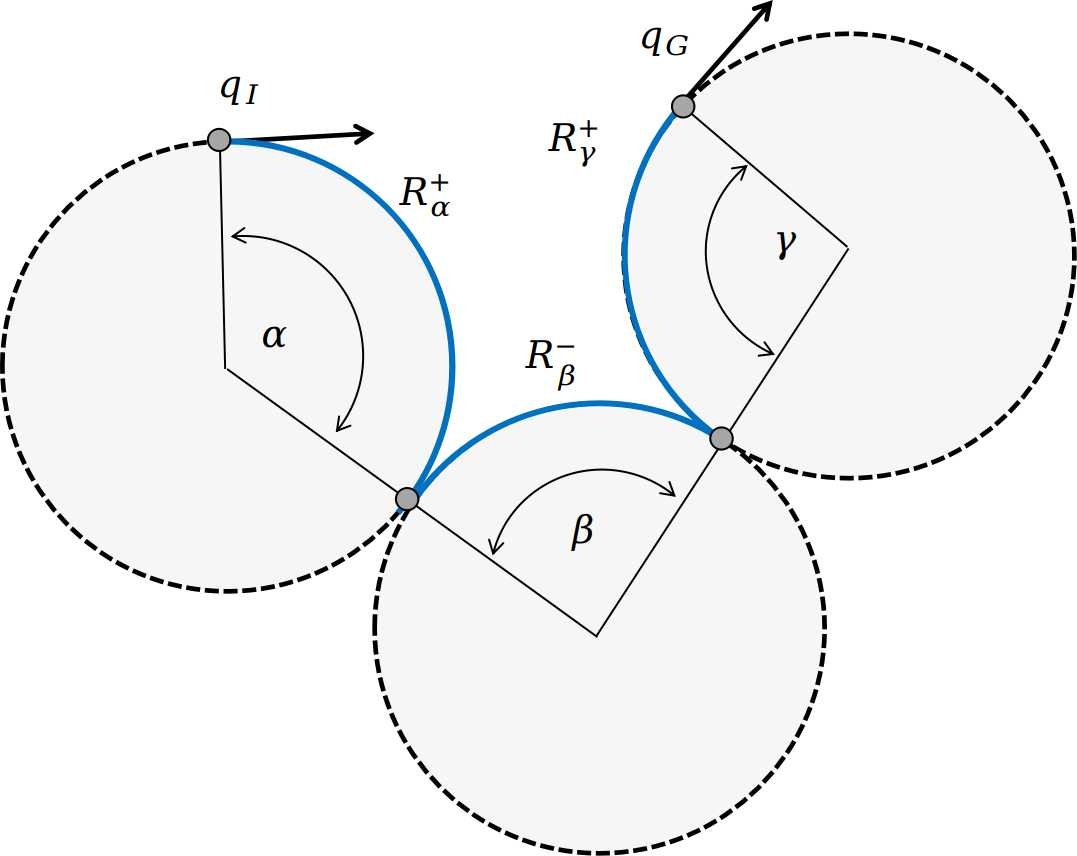
\includegraphics[width=9cm]{chapter04/RScurve.jpg}
  \bicaption[Reeds-Shepp曲线]
    {Reeds-Shepp曲线}
    {An example of Reeds-Shepp curve}
  \label{fig:rscurve}
\end{figure}


\subsubsection{碰撞检测}
我们用矩形包络船体,且用点、线段和最小边框(bounding box)表示周围的物体,
从而通过检测点、线段和最小边框是否与船体矩形重合来检测碰撞。


\subsubsection{A*算法}
A*搜索算法是一种在图形平面上,有多个节点的路径,求出最低通过成本的算法。
用于游戏中的NPC的移动计算,或网络游戏的BOT的移动计算上。
该算法综合了最良优先搜索和Dijkstra算法的优点:在进行启发式搜索提高算法效率的同时,
可以保证找到一条最优路径(基于评估函数)。在此算法中,如果以$g(n)$表示从起点到任意顶点$n$的实际距离,
$h(n)$表示任意顶点$n$到目标顶点的估算距离(根据所采用的评估函数的不同而变化),那么A*算法的估算函数为:

\begin{equation}
  f(n)=g(n)+h(n)
\end{equation}

这个公式遵循以下特性:
\begin{itemize}
  \item 
  如果$g(n)$为0,即只计算任意顶点$n$到目标的评估函数$h(n)$,
  而不计算起点到顶点$n$的距离,则算法转化为使用贪心策略的最良优先搜索,速度最快,但可能得不出最优解;
  \item 
  如果$h(n)$不大于顶点$n$到目标顶点的实际距离,则一定可以求出最优解,
  而且$h(n)$越小,需要计算的节点越多,算法效率越低,常见的评估函数有——欧几里得距离、曼哈顿距离、切比雪夫距离;
  \item 
  如果$h(n)$为0,即只需求出起点到任意顶点$n$的最短路径$g(n)$,而不计算任何评估函数$h(n)$, 
  则转化为单源最短路径问题,即Dijkstra算法,此时需要计算最多的顶点;
\end{itemize}


\subsubsection{混合A*搜索}
混合A*搜索算法(Hybrid A* search algorithm), 如图\ref{fig:manuverset}所示,


如图\ref{fig:HybridAstar}所示,



$\Delta \theta_{max}= \kappa_{max} L$


\begin{equation}
  \begin{aligned}
    & \Delta x = \frac{L}{\Delta \theta_{max}} 
    \left( \sin \Delta \theta_{max} \cos \theta - (1-\cos \Delta \theta_{max}) \sin \theta \right) \\
    & \Delta y = \frac{L}{\Delta \theta_{max}} 
    \left( \sin \Delta \theta_{max} \sin \theta + (1-\cos \Delta \theta_{max}) \cos \theta \right) 
  \end{aligned}
\end{equation}

\begin{figure}[!htp]
  \centering
  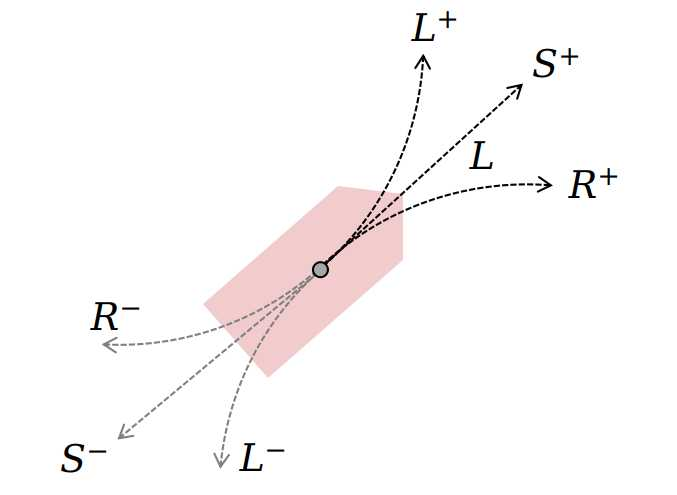
\includegraphics[width=9cm]{chapter04/manuverset.jpg}
  \bicaption[混合A*搜索算法中的可行操作模式]
    {混合A*搜索算法中的可行操作模式}
    {Manuver set of hybrid A* search algorithm}
  \label{fig:manuverset}
\end{figure}


\begin{figure}[!htp]
  \centering
  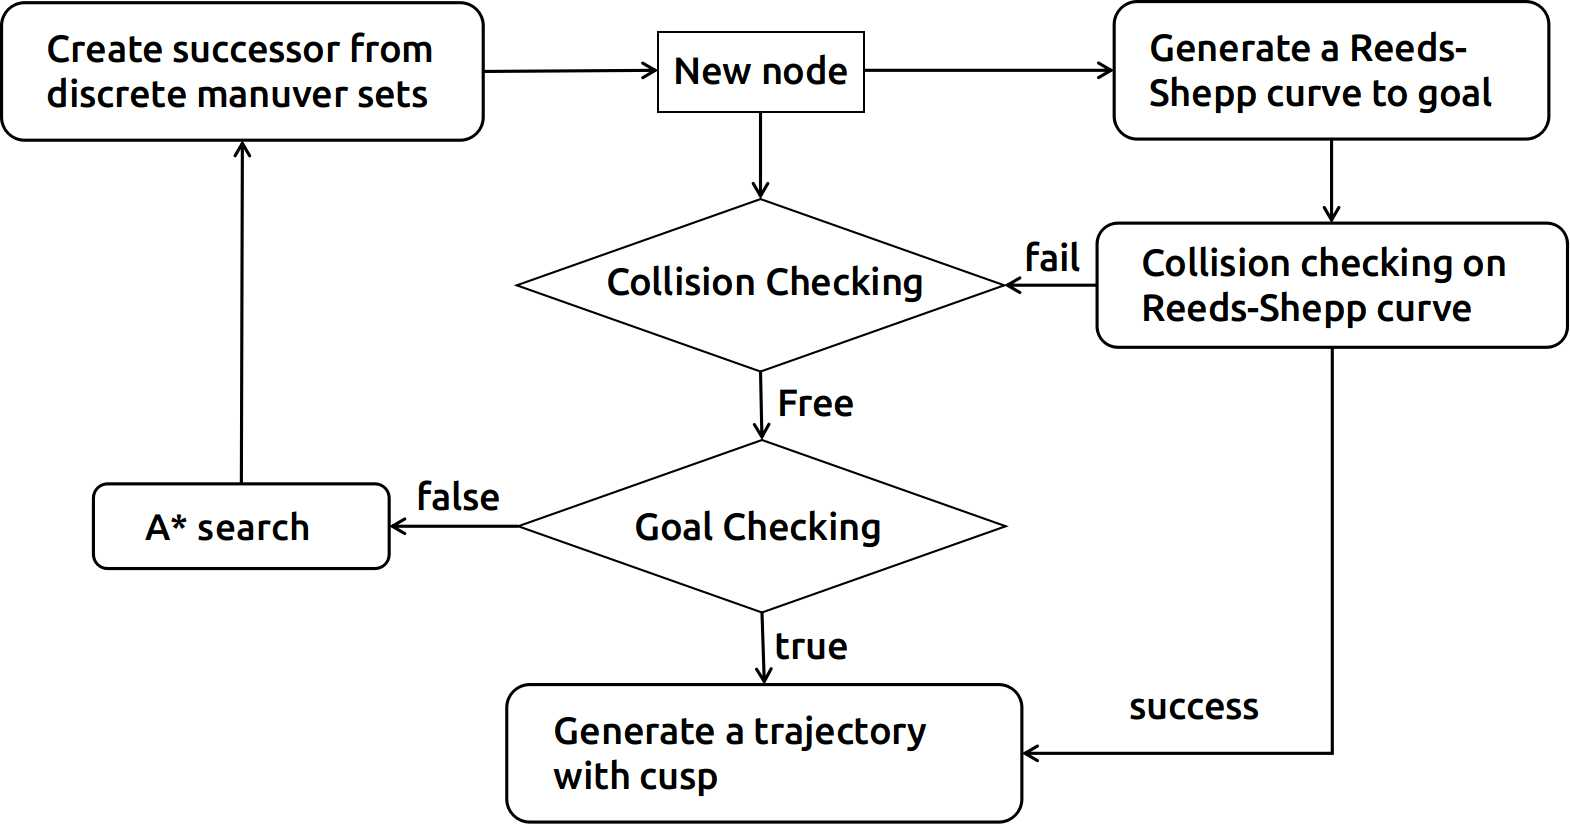
\includegraphics[width=14cm]{chapter04/HybridAstar.jpg}
  \bicaption[混合A*搜索算法]
    {混合A*搜索算法}
    {Hybrid A* search algorithm}
  \label{fig:HybridAstar}
\end{figure}

\subsubsection{轨迹平滑}
由A*算法生成的轨迹比较粗糙,需要通过平滑处理获得更好的轨迹。我们假定轨迹点为$\bm{x}_i=[x_i,y_i]$,如图\ref{fig:rscurve}
所示, 其中起点、终点和方向转换点保持不变$\Delta \bm{x}_{s}=0, \Delta \bm{x}_{sw}=0, \Delta \bm{x}_{e}=0$, 
剩下的轨迹点采用以下惩罚函数

\begin{equation} 
  \begin{aligned}
    F(\bm{x})
    &= \omega_s \sum_{i=1}^{e-1} ||\Delta \bm{x}_{i+1} - \Delta \bm{x}_{i}||_2^2 + \\
    &\omega_o \sum_{i=1}^{e-1} \sum_{j=1}^{N_i} \left( || \bm{x}_{i} - \bm{o}_{ij}||_2 - d_{max} \right)^2
     +\omega_k \sum_{i=1}^{e-1} 
     \left(\frac{\Delta \Phi_i }{|| \Delta \bm{x}_i ||_2} - \kappa_{max} \right)^2
  \end{aligned}
\end{equation}

其中,$\bm{o}_{ij}$为轨迹点$\bm{x}_i$在半径$d_{max}$之内的障碍物位置, 两点之间的位移
$\Delta \bm{x}_{i} = \bm{x}_i - \bm{x}_{i-1}$和夹角
\begin{equation} 
  \begin{aligned}
    \Delta \Phi_i
    &= | \arctan \frac{\Delta y_{i+1}}{\Delta x_{i+1}} - \arctan \frac{\Delta y_{i}}{\Delta x_{i}}| \\
    &= \arccos \frac{\Delta \bm{x}_i^T \Delta \bm{x}_{i+1} }
    {||\Delta \bm{x}_i||_2 ||\Delta \bm{x}_{i+1}||_2}
  \end{aligned}
\end{equation}

 $F_o$用于远离障碍物

\begin{equation} 
  \frac{\partial F_o}{\partial \bm{x}_i} = 2 \omega_o \sum_{j=1}^{N_i} 
  \left( || \bm{x}_{i} - \bm{o}_{ij}||_2 - d_{max} \right) \frac{\bm{x}_{i} - \bm{o}_{ij}}
  {|| \bm{x}_{i} - \bm{o}_{ij}||_2}
\end{equation}

\begin{figure}[!htp]
  \centering
  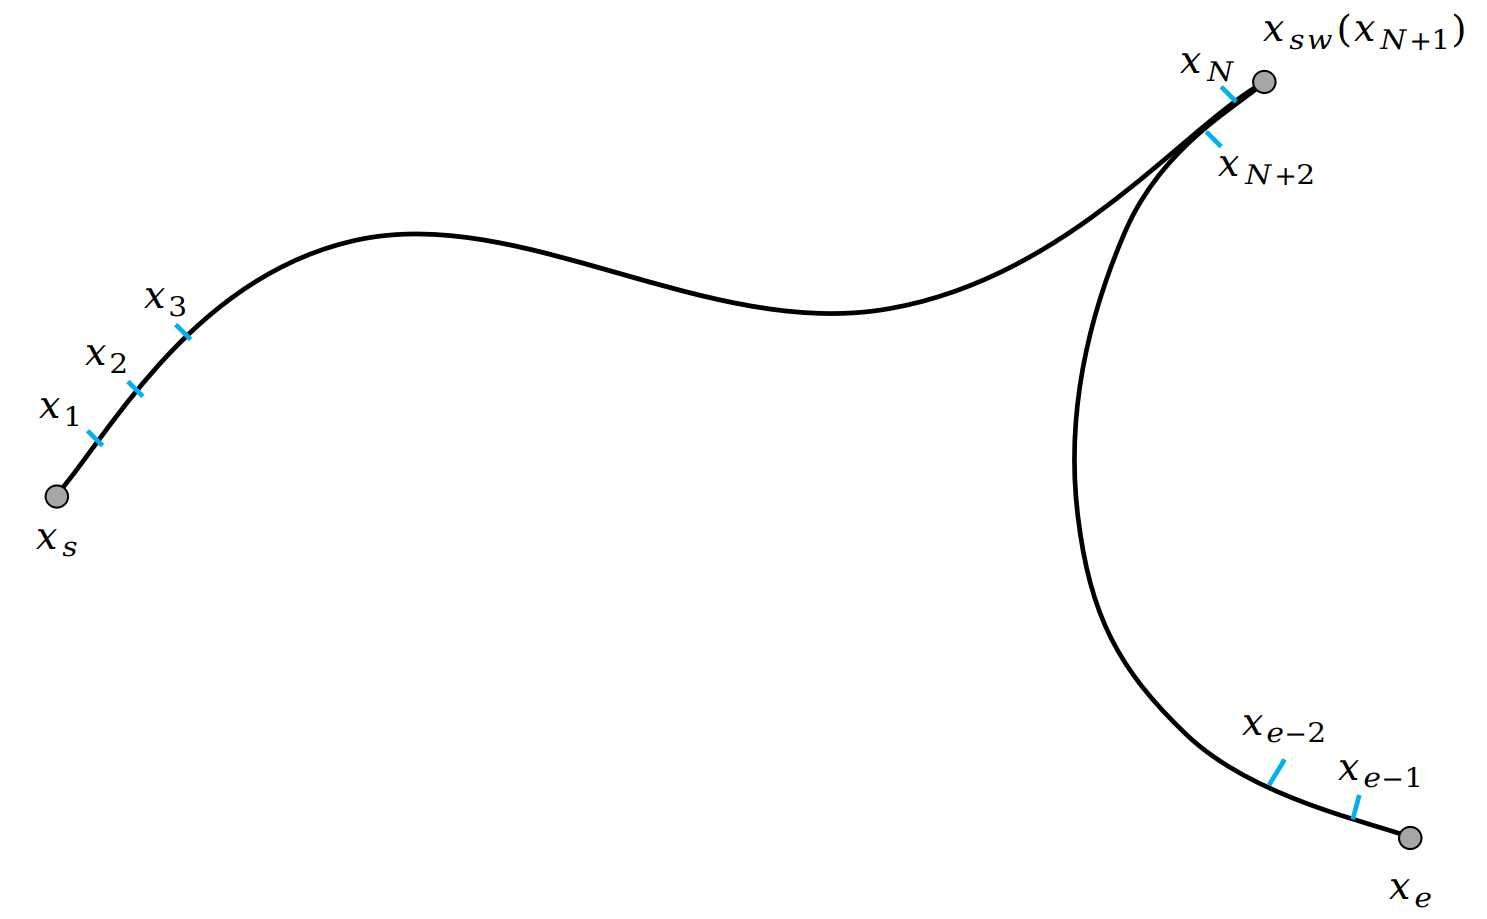
\includegraphics[width=14cm]{chapter04/pathsmoothing.jpg}
  \bicaption[轨迹平滑处理]
    {轨迹平滑处理}
    {Trajectory Smoothing}
  \label{fig:rscurve}
\end{figure}

对于$F_s$,表示轨迹的光滑性;
\begin{equation} 
  \begin{aligned}
    &\hat{\bm{x}}_i = \Delta \bm{x}_{i-1} -2 \Delta \bm{x}_i + \Delta \bm{x}_{i+1} \\
    &\frac{\partial F_s}{\partial \bm{x}_i} = 2 \omega_s 
    \left( \hat{\bm{x}}_{i-1} -2 \hat{\bm{x}}_{i} + \hat{\bm{x}}_{i+1}  \right) 
  \end{aligned}
\end{equation}
其中,起点$\hat{\bm{x}}_{i=s}=0$和终点$\hat{\bm{x}}_{i=e}=0$

$F_{\kappa}$用于惩罚过大的曲率,我们用$\kappa_i = \frac{\Delta \Phi_i }{|| \Delta \bm{x}_i ||_2} $表示轨迹点的曲率


\begin{equation} 
  \begin{aligned}
    \frac{\partial \kappa_i}{\partial \bm{x}_i} 
    &= \frac{1}{|| \Delta \bm{x}_i ||_2} \frac{\partial \Delta \Phi_i}{ \partial \cos(\Delta \Phi_i)}
    \frac{\partial \cos(\Delta \Phi_i)}{\partial \bm{x}_i} - 
    \frac{\Delta\Phi_i}{|| \Delta \bm{x}_i ||_2^2} \frac{\Delta \bm{x}_i}{|| \Delta \bm{x}_i ||_2}
    \\
    \frac{\partial \kappa_i}{\partial \bm{x}_{i-1}} 
    &=\frac{1}{|| \Delta \bm{x}_i ||_2} \frac{\partial \Delta \Phi_i}{ \partial \cos(\Delta \Phi_i)}
    \frac{\partial \cos(\Delta \Phi_i)}{\partial \bm{x}_{i-1}} +  
    \frac{\Delta\Phi_i}{|| \Delta \bm{x}_i ||_2^2} \frac{\Delta \bm{x}_i}{|| \Delta \bm{x}_i ||_2} 
    \\
    \frac{\partial \kappa_i}{\partial \bm{x}_{i+1}} 
    &=\frac{1}{|| \Delta \bm{x}_i ||_2} \frac{\partial \Delta \Phi_i}{ \partial \cos(\Delta \Phi_i)}
        \frac{\partial \cos(\Delta \Phi_i)}{\partial \bm{x}_{i+1}} \\
  \end{aligned}
\end{equation}
其中
\begin{equation} 
  \frac{\partial \Delta \Phi_i}{ \partial \cos(\Delta \Phi_i)} = 
  \frac{-1}{\left( 1-\cos^2(\Delta \Phi_i) \right)^{1/2}}
\end{equation}
我们引入正交补(orthogonal complements)
\begin{equation} 
   \bm{a} \perp \bm{b}= \bm{a} - \frac{ \bm{a}^T \bm{b}}{|\bm{b}|} \frac{\bm{b}}{|\bm{b}|}
\end{equation}

用于表示
\begin{equation} 
   \bm{P}_1 = \frac{ \Delta \bm{x}_i \perp (-\Delta \bm{x}_{i+1})}
   {||\Delta \bm{x}_i||_2 ||\Delta \bm{x}_{i+1}||_2} ; \quad 
   \bm{P}_2 = \frac{ (-\Delta \bm{x}_{i+1}) \perp \Delta \bm{x}_i }
   {||\Delta \bm{x}_i||_2 ||\Delta \bm{x}_{i+1}||_2} 
\end{equation}

从而
\begin{equation} 
   \frac{\partial \cos(\Delta \Phi_i)}{\partial \bm{x}_i} = -\bm{P}_1 - \bm{P}_2; \quad
   \frac{\partial \cos(\Delta \Phi_i)}{\partial \bm{x}_{i-1}} = \bm{P}_2; \quad
   \frac{\partial \cos(\Delta \Phi_i)}{\partial \bm{x}_{i+1}} = \bm{P}_1. 
\end{equation}


\begin{equation} 
  \Delta \hat{\Phi}_i= \frac{\Delta \Phi_i}{|| \bm{x}_i - \bm{x}_{i-1}||_2}; \;
  \hat{P}_1^i= \frac{\bm{P}_1^i}{|| \bm{x}_i - \bm{x}_{i-1}||_2 \sin \Delta \Phi_i}; \; 
  \hat{P}_2^i= \frac{\bm{P}_2^i}{|| \bm{x}_i - \bm{x}_{i-1}||_2 \sin \Delta \Phi_i}.
\end{equation}
对于起点($i=s$)和终点($i=e$),$\Delta \hat{\Phi}_i=0, \hat{P}_1^i=\hat{P}_2^i=0$。

\begin{equation} 
  \begin{aligned}
    \frac{\partial F_k}{\partial \bm{x}_i }
    = 2 \omega_k \Bigg[
    &(\Delta \hat{\Phi}_{i-1}-\kappa_{max}) \left(-\hat{\bm{P}}_1^{i-1} \right) +  \\
    &(\Delta \hat{\Phi}_{i}-\kappa_{max}) \left( \hat{\bm{P}}_1^{i}+\hat{\bm{P}}_2^{i}
    -\Delta \hat{\Phi}_i \frac{\bm{x}_i-\bm{x}_{i-1}}{||\bm{x}_i-\bm{x}_{i-1}||_2^2} \right) + \\
    &(\Delta \hat{\Phi}_{i+1}-\kappa_{max}) \left( -\hat{\bm{P}}_1^{i+1} + 
    \Delta \hat{\Phi}_{i+1} \frac{\bm{x}_{i+1}-\bm{x}_i}{||\bm{x}_{i+1}-\bm{x}_i||_2^2} \right)
    \Bigg]
  \end{aligned}
\end{equation}

当我们得到了当前轨迹的梯度$\nabla F(\bm{x})$, 使得下降方向$\Delta \bm{x}=-\nabla F(\bm{x})$, 需要选择一个
$t$, 使得$F( \bm{x} + t \Delta \bm{x})< F(\bm{x})$, 这时可采用回溯线搜索(backtracking line search)计算得到该$t$。
给定$\alpha \in (0,1/2), \beta \in (0,1)$, 初始$t=1$, 重复$t:=\beta t$, 直到

\begin{equation} 
  F(\bm(x)+t \Delta \bm{x}) < F(\bm{x}) + \alpha t \nabla F(\bm{x})^T \Delta \bm{x}
\end{equation}



\section{航线规划}
\label{sec:routeplanning}

A*算法

\section{行为规划}
\label{sec:behav}
